%%%%%%%%%%%%%%%%%%%%%%%%%%%%%%%%%%%%%%%%%%%%%%%%%%%%%%%%%%%%%%%
%% OXFORD THESIS TEMPLATE

% Use this template to produce a standard thesis that meets the Oxford University requirements for DPhil submission
%
% Originally by Keith A. Gillow (gillow@maths.ox.ac.uk), 1997
% Modified by Sam Evans (sam@samuelevansresearch.org), 2007
% Modified by John McManigle (john@oxfordechoes.com), 2015
%
% This version Copyright (c) 2015-2017 John McManigle
%
% Broad permissions are granted to use, modify, and distribute this software
% as specified in the MIT License included in this distribution's LICENSE file.
%

% I've (John) tried to comment this file extensively, so read through it to see how to use the various options.  Remember
% that in LaTeX, any line starting with a % is NOT executed.  Several places below, you have a choice of which line to use
% out of multiple options (eg draft vs final, for PDF vs for binding, etc.)  When you pick one, add a % to the beginning of
% the lines you don't want.


%%%%% CHOOSE PAGE LAYOUT
% The most common choices should be below.  You can also do other things, like replacing "a4paper" with "letterpaper", etc.

% This one will format for two-sided binding (ie left and right pages have mirror margins; blank pages inserted where needed):
\documentclass[a4paper,twoside]{ociamthesis}
% This one will format for one-sided binding (ie left margin > right margin; no extra blank pages):
%\documentclass[a4paper]{ociamthesis}
% This one will format for PDF output (ie equal margins, no extra blank pages):
%\documentclass[a4paper,nobind]{ociamthesis} 



%%%%% SELECT YOUR DRAFT OPTIONS
% Three options going on here; use in any combination.  But remember to turn the first two off before
% generating a PDF to send to the printer!

% This adds a "DRAFT" footer to every normal page.  (The first page of each chapter is not a "normal" page.)
\fancyfoot[C]{\emph{DRAFT Printed on \today}}  

% This highlights (in blue) corrections marked with (for words) \mccorrect{blah} or (for whole
% paragraphs) \begin{mccorrection} . . . \end{mccorrection}.  This can be useful for sending a PDF of
% your corrected thesis to your examiners for review.  Turn it off, and the blue disappears.
\correctionstrue


%%%%% BIBLIOGRAPHY SETUP
% Note that your bibliography will require some tweaking depending on your department, preferred format, etc.
% The options included below are just very basic "sciencey" and "humanitiesey" options to get started.
% If you've not used LaTeX before, I recommend reading a little about biblatex/biber and getting started with it.
% If you're already a LaTeX pro and are used to natbib or something, modify as necessary.
% Either way, you'll have to choose and configure an appropriate bibliography format...

% The science-type option: numerical in-text citation with references in order of appearance.
\usepackage[style=numeric-comp, sorting=none, backend=biber, doi=false, isbn=false]{biblatex}
\newcommand*{\bibtitle}{References}

% The humanities-type option: author-year in-text citation with an alphabetical works cited.
%\usepackage[style=authoryear, sorting=nyt, backend=biber, maxcitenames=2, useprefix, doi=false, isbn=false]{biblatex}
%\newcommand*{\bibtitle}{Works Cited}

% This makes the bibliography left-aligned (not 'justified') and slightly smaller font.
\renewcommand*{\bibfont}{\raggedright\small}

% Change this to the name of your .bib file (usually exported from a citation manager like Zotero or EndNote).
\addbibresource{references.bib}


% Uncomment this if you want equation numbers per section (2.3.12), instead of per chapter (2.18):
%\numberwithin{equation}{subsection}



%%%%% THESIS / TITLE PAGE INFORMATION
% Everybody needs to complete the following:
\title{Suitably impressive thesis title}
\author{Your Name}
\college{Your College}

% Master's candidates who require the alternate title page (with candidate number and word count)
% must also un-comment and complete the following three lines:
%\masterssubmissiontrue
%\candidateno{933516}
%\wordcount{28,815}

% Uncomment the following line if your degree also includes exams (eg most masters):
%\renewcommand{\submittedtext}{Submitted in partial completion of the}
% Your full degree name.  (But remember that DPhils aren't "in" anything.  They're just DPhils.)
\degree{Doctor of Philosophy}
% Term and year of submission, or date if your board requires (eg most masters)
\degreedate{Michaelmas 2014}


%%%%% YOUR OWN PERSONAL MACROS
% This is a good place to dump your own LaTeX macros as they come up.

% To make text superscripts shortcuts
	\renewcommand{\th}{\textsuperscript{th}}
	\newcommand{\nd}{\textsuperscript{nd}}
	\renewcommand{\st}{\textsuperscript{st}}
	\newcommand{\rd}{\textsuperscript{rd}}
	\newcommand{\uL}{$\mu$L }
    \newcommand{\uM}{$\mu$M }
    \newcommand{\ug}{$\mu$g }
	\newcommand{\R}{\textsuperscript{\textregistered} }

%%%%% THE ACTUAL DOCUMENT STARTS HERE
\begin{document}



%%%%% CHOOSE YOUR LINE SPACING HERE
% This is the official option.  Use it for your submission copy and library copy:
\setlength{\textbaselineskip}{22pt plus2pt}
% This is closer spacing (about 1.5-spaced) that you might prefer for your personal copies:
%\setlength{\textbaselineskip}{18pt plus2pt minus1pt}

% You can set the spacing here for the roman-numbered pages (acknowledgements, table of contents, etc.)
\setlength{\frontmatterbaselineskip}{17pt plus1pt minus1pt}

% Leave this line alone; it gets things started for the real document.
\setlength{\baselineskip}{\textbaselineskip}


%%%%% CHOOSE YOUR SECTION NUMBERING DEPTH HERE
% You have two choices.  First, how far down are sections numbered?  (Below that, they're named but
% don't get numbers.)  Second, what level of section appears in the table of contents?  These don't have
% to match: you can have numbered sections that don't show up in the ToC, or unnumbered sections that
% do.  Throughout, 0 = chapter; 1 = section; 2 = subsection; 3 = subsubsection, 4 = paragraph...

% The level that gets a number:
\setcounter{secnumdepth}{2}
% The level that shows up in the ToC:
\setcounter{tocdepth}{2}


%%%%% ABSTRACT SEPARATE
% This is used to create the separate, one-page abstract that you are required to hand into the Exam
% Schools.  You can comment it out to generate a PDF for printing or whatnot.
\begin{abstractseparate}
	

Lorem ipsum dolor sit amet, consectetur adipiscing elit. Pellentesque sit amet nibh volutpat, scelerisque nibh a, vehicula neque. Integer placerat nulla massa, et vestibulum velit dignissim id. Ut eget nisi elementum, consectetur nibh in, condimentum velit. Quisque sodales dui ut tempus mattis. Duis malesuada arcu at ligula egestas egestas. Phasellus interdum odio at sapien fringilla scelerisque. Mauris sagittis eleifend sapien, sit amet laoreet felis mollis quis. Pellentesque dui ante, finibus eget blandit sit amet, tincidunt eu neque. Vivamus rutrum dapibus ligula, ut imperdiet lectus tincidunt ac. Pellentesque ac lorem sed diam egestas lobortis.

Suspendisse leo purus, efficitur mattis urna a, maximus molestie nisl. Aenean porta semper tortor a vestibulum. Suspendisse viverra facilisis lorem, non pretium erat lacinia a. Vestibulum tempus, quam vitae placerat porta, magna risus euismod purus, in viverra lorem dui at metus. Sed ac sollicitudin nunc. In maximus ipsum nunc, placerat maximus tortor gravida varius. Suspendisse pretium, lorem at porttitor rhoncus, nulla urna condimentum tortor, sed suscipit nisi metus ac risus.

Aenean sit amet enim quis lorem tristique commodo vitae ut lorem. Duis vel tincidunt lacus. Sed massa velit, lacinia sed posuere vitae, malesuada vel ante. Praesent a rhoncus leo. Etiam sed rutrum enim. Pellentesque lobortis elementum augue, at suscipit justo malesuada at. Lorem ipsum dolor sit amet, consectetur adipiscing elit. Praesent rhoncus convallis ex. Etiam commodo nunc ex, non consequat diam consectetur ut. Pellentesque vitae est nec enim interdum dapibus. Donec dapibus purus ipsum, eget tincidunt ex gravida eget. Donec luctus nisi eu fringilla mollis. Donec eget lobortis diam.

Suspendisse finibus placerat dolor. Etiam ornare elementum ex ut vehicula. Donec accumsan mattis erat. Quisque cursus fringilla diam, eget placerat neque bibendum eu. Ut faucibus dui vitae dolor porta, at elementum ipsum semper. Sed ultrices dui non arcu pellentesque placerat. Etiam posuere malesuada turpis, nec malesuada tellus malesuada. % Create an abstract.tex file in the 'text' folder for your abstract.
\end{abstractseparate}


% JEM: Pages are roman numbered from here, though page numbers are invisible until ToC.  This is in
% keeping with most typesetting conventions.
\begin{romanpages}

% Title page is created here
\maketitle

%%%%% DEDICATION -- If you'd like one, un-comment the following.
%\begin{dedication}
%This thesis is dedicated to\\
%someone\\
%for some special reason\\
%\end{dedication}

%%%%% ACKNOWLEDGEMENTS -- Nothing to do here except comment out if you don't want it.
\begin{acknowledgements}
 	\input{text/acknowledgements}
\end{acknowledgements}

%%%%% ABSTRACT -- Nothing to do here except comment out if you don't want it.
\begin{abstract}
	

Lorem ipsum dolor sit amet, consectetur adipiscing elit. Pellentesque sit amet nibh volutpat, scelerisque nibh a, vehicula neque. Integer placerat nulla massa, et vestibulum velit dignissim id. Ut eget nisi elementum, consectetur nibh in, condimentum velit. Quisque sodales dui ut tempus mattis. Duis malesuada arcu at ligula egestas egestas. Phasellus interdum odio at sapien fringilla scelerisque. Mauris sagittis eleifend sapien, sit amet laoreet felis mollis quis. Pellentesque dui ante, finibus eget blandit sit amet, tincidunt eu neque. Vivamus rutrum dapibus ligula, ut imperdiet lectus tincidunt ac. Pellentesque ac lorem sed diam egestas lobortis.

Suspendisse leo purus, efficitur mattis urna a, maximus molestie nisl. Aenean porta semper tortor a vestibulum. Suspendisse viverra facilisis lorem, non pretium erat lacinia a. Vestibulum tempus, quam vitae placerat porta, magna risus euismod purus, in viverra lorem dui at metus. Sed ac sollicitudin nunc. In maximus ipsum nunc, placerat maximus tortor gravida varius. Suspendisse pretium, lorem at porttitor rhoncus, nulla urna condimentum tortor, sed suscipit nisi metus ac risus.

Aenean sit amet enim quis lorem tristique commodo vitae ut lorem. Duis vel tincidunt lacus. Sed massa velit, lacinia sed posuere vitae, malesuada vel ante. Praesent a rhoncus leo. Etiam sed rutrum enim. Pellentesque lobortis elementum augue, at suscipit justo malesuada at. Lorem ipsum dolor sit amet, consectetur adipiscing elit. Praesent rhoncus convallis ex. Etiam commodo nunc ex, non consequat diam consectetur ut. Pellentesque vitae est nec enim interdum dapibus. Donec dapibus purus ipsum, eget tincidunt ex gravida eget. Donec luctus nisi eu fringilla mollis. Donec eget lobortis diam.

Suspendisse finibus placerat dolor. Etiam ornare elementum ex ut vehicula. Donec accumsan mattis erat. Quisque cursus fringilla diam, eget placerat neque bibendum eu. Ut faucibus dui vitae dolor porta, at elementum ipsum semper. Sed ultrices dui non arcu pellentesque placerat. Etiam posuere malesuada turpis, nec malesuada tellus malesuada.
\end{abstract}

%%%%% MINI TABLES
% This lays the groundwork for per-chapter, mini tables of contents.  Comment the following line
% (and remove \minitoc from the chapter files) if you don't want this.  Un-comment either of the
% next two lines if you want a per-chapter list of figures or tables.
\dominitoc % include a mini table of contents
%\dominilof  % include a mini list of figures
%\dominilot  % include a mini list of tables

% This aligns the bottom of the text of each page.  It generally makes things look better.
\flushbottom

% This is where the whole-document ToC appears:
\tableofcontents

\listoffigures
	\mtcaddchapter
% \mtcaddchapter is needed when adding a non-chapter (but chapter-like) entity to avoid confusing minitoc

% Uncomment to generate a list of tables:
%\listoftables
%	\mtcaddchapter

%%%%% LIST OF ABBREVIATIONS
% This example includes a list of abbreviations.  Look at text/abbreviations.tex to see how that file is
% formatted.  The template can handle any kind of list though, so this might be a good place for a
% glossary, etc.
% First parameter can be changed eg to "Glossary" or something.
% Second parameter is the max length of bold terms.
\begin{mclistof}{List of Abbreviations}{3.2cm}

\item[CVD] Cardiovascular disease

\item[DNL] \textit{De novo} lipogenesis

\item[GLY] Glycogenolysis

\item[GNG] Gluconeogenesis

\item[IHTG] Intrahepatic triglyceride

\item[IR] Insulin resistance/insulin resistant

\item[NAFLD] Nonalcoholic fatty liver disease (also known as metabolic associated fatty liver disease (MAFLD))

\item[NEFA] Non-esterified fatty acid

\item[PCR] Polymerase chain reaction

\item[T2D] Type II diabetes mellitus 

\item[TG] Triglyceride

\end{mclistof} 


% The Roman pages, like the Roman Empire, must come to its inevitable close.
\end{romanpages}


%%%%% CHAPTERS
% Add or remove any chapters you'd like here, by file name (excluding '.tex'):
\flushbottom
\chapter{\label{ch:1-background}Background} 

\minitoc

\section{Obesity}

In 2016 the World Health Organisation estimated 1.9 billion adults worldwide were classified as overweight, with 650 million of these classified as obese  \cite{WHO2016factsheetObesityOverweight}, and the prevalence has continued to increase rapidly \cite{WHO2016factsheetObesityOverweight, Finucane2011NationalParticipants}. Obesity is a major risk factor for insulin resistance (IR), type-2 diabetes mellitus (T2D) and cardiovascular disease (CVD) \cite{Reaven1995PathophysiologyDisease, DeFronzo2015TypeMellitus, Khan2018AssociationMorbidity}; it is strongly associated with fat deposition in non-adipose tissue organs (ectopic fat), including the liver, heart, and skeletal muscle.

\section{The liver}

\subsection{Structure}

Anatomically the liver can be split into four main lobes that consist of small hexagonal lobules containing the four cell types: 1) sinusoidal endothelial cells, 2) stellate cells, 3) Kupffer cells, and 4) hepatocytes. Along each corner of the lobule there is the portal triad made up of the hepatic artery, the hepatic portal vein, and the common bile duct. As well as the oxygen-rich blood from the hepatic artery, the liver is unique in that it also receives nutrient-rich deoxygenated blood directly from the pancreas, spleen and the entire gastrointestinal tract through the hepatic portal vein. The blood from both vessels combine in the liver sinusoid and travel down to a central vein in the middle of each lobule which will eventually drain into the hepatic vein and then the inferior vena cava. The liver sinusoid is lined with sinusoidal endothelial cells and liver-specific tissue-resident macrophages known as Kuppfer cells which remove debris and foreign particles through phagocytosis. The endothelial cells are highly fenestrated, which allows communication between the sinusoid and the hepatocytes and stellate cells.

\subsection{Function}

The liver has many hundreds of functions, including the production of bile, regulation of systemic iron levels, synthesis of amino acids and cholesterol, regulation of blood clotting and detoxification of the blood. One of the main functions is the regulation and metabolism of key nutritional substrates in the blood such as glucose and fatty acids. These processes are primarily under the control of pancreatic hormones insulin and glucagon which the liver gets the first pass of and are themselves regulated by nutritional state.  

\subsubsection{Glucose Metabolism}

In the fasting state blood glucose is maintained by endogenous glucose production which occurs almost exclusively in the liver. Glycogen stores are broken down into glucose through glycogenolysis (GLY) and new glucose molecules are made from non-carbohydrate precursors (such as amino acids and glycerol) through gluconeogenesis (GNG). An increase in glucagon and decrease in insulin levels in the blood is responsible for this up-regulation of GNG and GLY. In the transition to the postprandial state after the consumption of a mixed meal, glucagon secretion is inhibited and plasma insulin concentrations sharply rise. This shifts hepatic metabolism to a decrease in glucose production and an increase in glucose uptake, storage and oxidation. 

\subsubsection{Fatty Acid Metabolism}


Triglyceride (TG) is a crucial metabolic substrate for many parts of the body. TG can be synthesised in the liver from non-lipid precursors through a process called \textit{de novo} lipogeneis (DNL) where it is then stored in lipid droplets(LD) or secreted packaged in TG-enriched very low-density lipoprotein (VLDL-TG). DNL is up-regulated by the presence of excess carbohydrates as well as the hormone insulin. 

\section{Non-alcoholic fatty liver disease}

\section{Autophagy}
\chapter{\label{ch:2-Methods}Methods}

\minitoc

\section{Cell culture procedures}

\subsection{Routine cell culture}

Human hepatocellular carcinoma cells (Huh7) were kindly provided by Dr Camilla Pramfalk (Karolinska Institutet) and human hepatic stellate cells (LX2) by Hamish Miller (Blizard Institute). Cells were cultured in maintenance media made from Dulbecco's modified Eagle's medium (DMEM) supplemented with GlutaMAX\textsuperscript{TM}, 5.5 mmol/L glucose, 1 mM sodium pyruvate, 2.4 g/L sodium bicarbonate, 10\% foetal bovine serum (FBS), 10,000 U/ml penicillin-streptomycin (P/S) and 1\% non-essential amino acids (NEAA). Maintenance media was changed every 2-3 days and cells kept in a incubator at 37\textdegree C and 5\% carbon dioxide. 

\subsection{Passaging cells}

Cells were grown to at least 80\% confluence in T175 (175 cm\textsuperscript{2}) flasks before being washed with phosphate buffered saline (PBS) and then incubated for 5 mins in 4-5 mL of TrypLE\textsuperscript{TM}. Flasks were then agitated to dislodge cells and 8 mL of maintenance media was added. Cells were centrifuged for at 800 rpm for 3 mins at 21\textdegree C. The supernatant was removed and the pellet re-suspended in 5 mL of maintenance media before being seeded 1:5 in new T175 flasks with maintenance media.

\subsection{Seeding cells for experiments}

Cells were isolated and re-suspended in maintenance media as described for passaging. 20 \uL of cells were added to both sides of a cell counter slide and cells were counted using a Cellometer Auto T4 Bright Field Cell Counter. An average of both sides was taken and cells were then diluted with maintenance media to a concentration of 1 x 10\textsuperscript{5} cells per mL. Total cell number per well were as follows: 6-well plate - 2 x 10\textsuperscript{5}, 12-well plate - 1 x 10\textsuperscript{5}, 24-well plate - 0.5 x 10\textsuperscript{5}, 96-well plate - 0.1 x 10\textsuperscript{5}.

\subsection{Freezing cells for storage in liquid nitrogen}

During passaging, cells were isolated but resuspended in 10 mL freezing media made from 90\% maintenance media and 10\% dimethyl sulfoxide (DMSO). 1 mL of the cell suspension was placed into each cryovial before being stored overnight in a -80\textdegree C freezer in a Styrofoam holder to slow the rate of cooling. Cells were then transferred to liquid nitrogen for long-term storage.  

\subsection{Thawing cells from storage in liquid nitrogen}

Frozen cells were placed in a 37\textdegree C water bath to thaw rapidly. 500 \uL of warm maintenance media was then added to the cryovial and mixed with a pipette. Cells were then seeded in a T75 (75cm\textsuperscript{2}) flask with maintenance media. Media was changed the next day and then every other day until cells reached at least 80\% and were passaged into a T175 flask.

\section {Quantitative reverse-transcription PCR}

\subsection{RNA extraction}

Cells for were cultured in 12-well plates and upon harvesting were washed twice with warm PBS before 250 \uL of TRI Reagent\textsuperscript{\textregistered}  was added to each well. Cells were dislodged from the plate using a cell scraper and transferred into Eppendorf tubes to be frozen at -80\textdegree C until required. When required, samples were added to Phase Lock Gel tubes with 50 \uL of chloroform and shaken vigorously. Samples were left for 5 mins and then centrifuged for 15 mins at 1200 g and 4\textdegree C. The clear supernatant was transferred to 2 mL tapered-bottom elution tubes containing 2 \uL glycol blue and 200 \uL isopropanol before being left overnight at -20\textdegree C. 

Samples were then centrifuged at 1200 g and 4\textdegree C for 30 mins to allow a RNA pellet to form. The supernatant was removed and pellet resuspended in 80\% ethanol before being centrifuged again at 1200 g and 4\textdegree C for 15 mins. The ethanol was then removed and the pellet allowed to dry before re-suspension in 15 \uL RNAse free water and incubation for 3 hours. RNA purity and concentration was then measured using a NanoDrop ND-1000 Spectrophotometer.

\subsection{Reverse transcription}

The volume of sample containing 1 \ug RNA was transferred into a 96 well plate and made up to 10 \uL with RNAse-free water. For each well with sample, 2 \uL 10x reverse transcription buffer, 0.8 \uL 25x deoxynucleoside triphosphates (dNTPs), 2 \uL 10x random primers, 1 \uL reverse transcriptase and 4.2 \uL RNAse-free water was added. The plate was sealed and briefly spun before being placed on an MJ Research Tetrad PTC-225 Thermal Cycler. The thermal cycler heated the plate to 27 \textdegree C for 10 minutes for the random primers to anneal to the sample RNA and this was then followed by 120 minutes at 37\textdegree C for the reverse transcriptase to form the cDNA using the dNTPs. Finally the reaction was terminated by heating the plate to 85\textdegree C for 5 mins. The cDNA could then be stored in the freezer until required. 

\subsection{Quantative PCR}

The samples were diluted 1:40 in 10 mmol/L Trizma\R hydrochloride and measured in triplicate for each gene. A standard curve was made through serial dilution of cDNA pooled from all of the samples in 10 mmol/L Trizma\R and included for each gene. Quantative PCR was carried out on \textbf{Insert name of machine} and TaqMan\R assays used to measure gene expression. A 6 \uL reaction volume was used consisting of 2.7 \uL of sample cDNA, 0.3 \uL TaqMan\R probes and 3 \uL 2X KAPA PROBE FAST Master Mix. Relative expression was calculated as a ratio from generated Ct values as previously described \cite{Pfaffl2001ARTPCR}. Each sample was expressed relative to a calibrator sample and corrected to the geometric mean of three reference housekeeper genes (B2M, HMBS, and YWHAZ).
\chapter{\label{ch:3-Model Development}Model Development}

\minitoc

 \section{Introduction}

 \section{Methods}

 \section{Results}

\subsection{Effect of media FA concentration on TG accumulation and autophagy}

By culturing Huh7 cells in increasing concentrations of OPLA FA mix, intracellular TG content significantly increased (Figure \ref{fig:LFHF TG}) but despite the substantial increase in TG accumulation, there was no effect on autophagic gene expression (Figure \ref{fig:LFHF ATG genes}).

\begin{figure}[h!]
  \centering
  {\phantomsubcaption\label{fig:LFHF TG}}
  {\phantomsubcaption\label{fig:LFHF ATG genes}}
   {\phantomsubcaption\label{fig:OPLA 0uM Picture}}
    {\phantomsubcaption\label{fig:OPLA 800uM Picture}}
  \tikz\node[inner sep=0pt,label={[anchor=north west]north west:\subref{fig:LFHF TG}}] {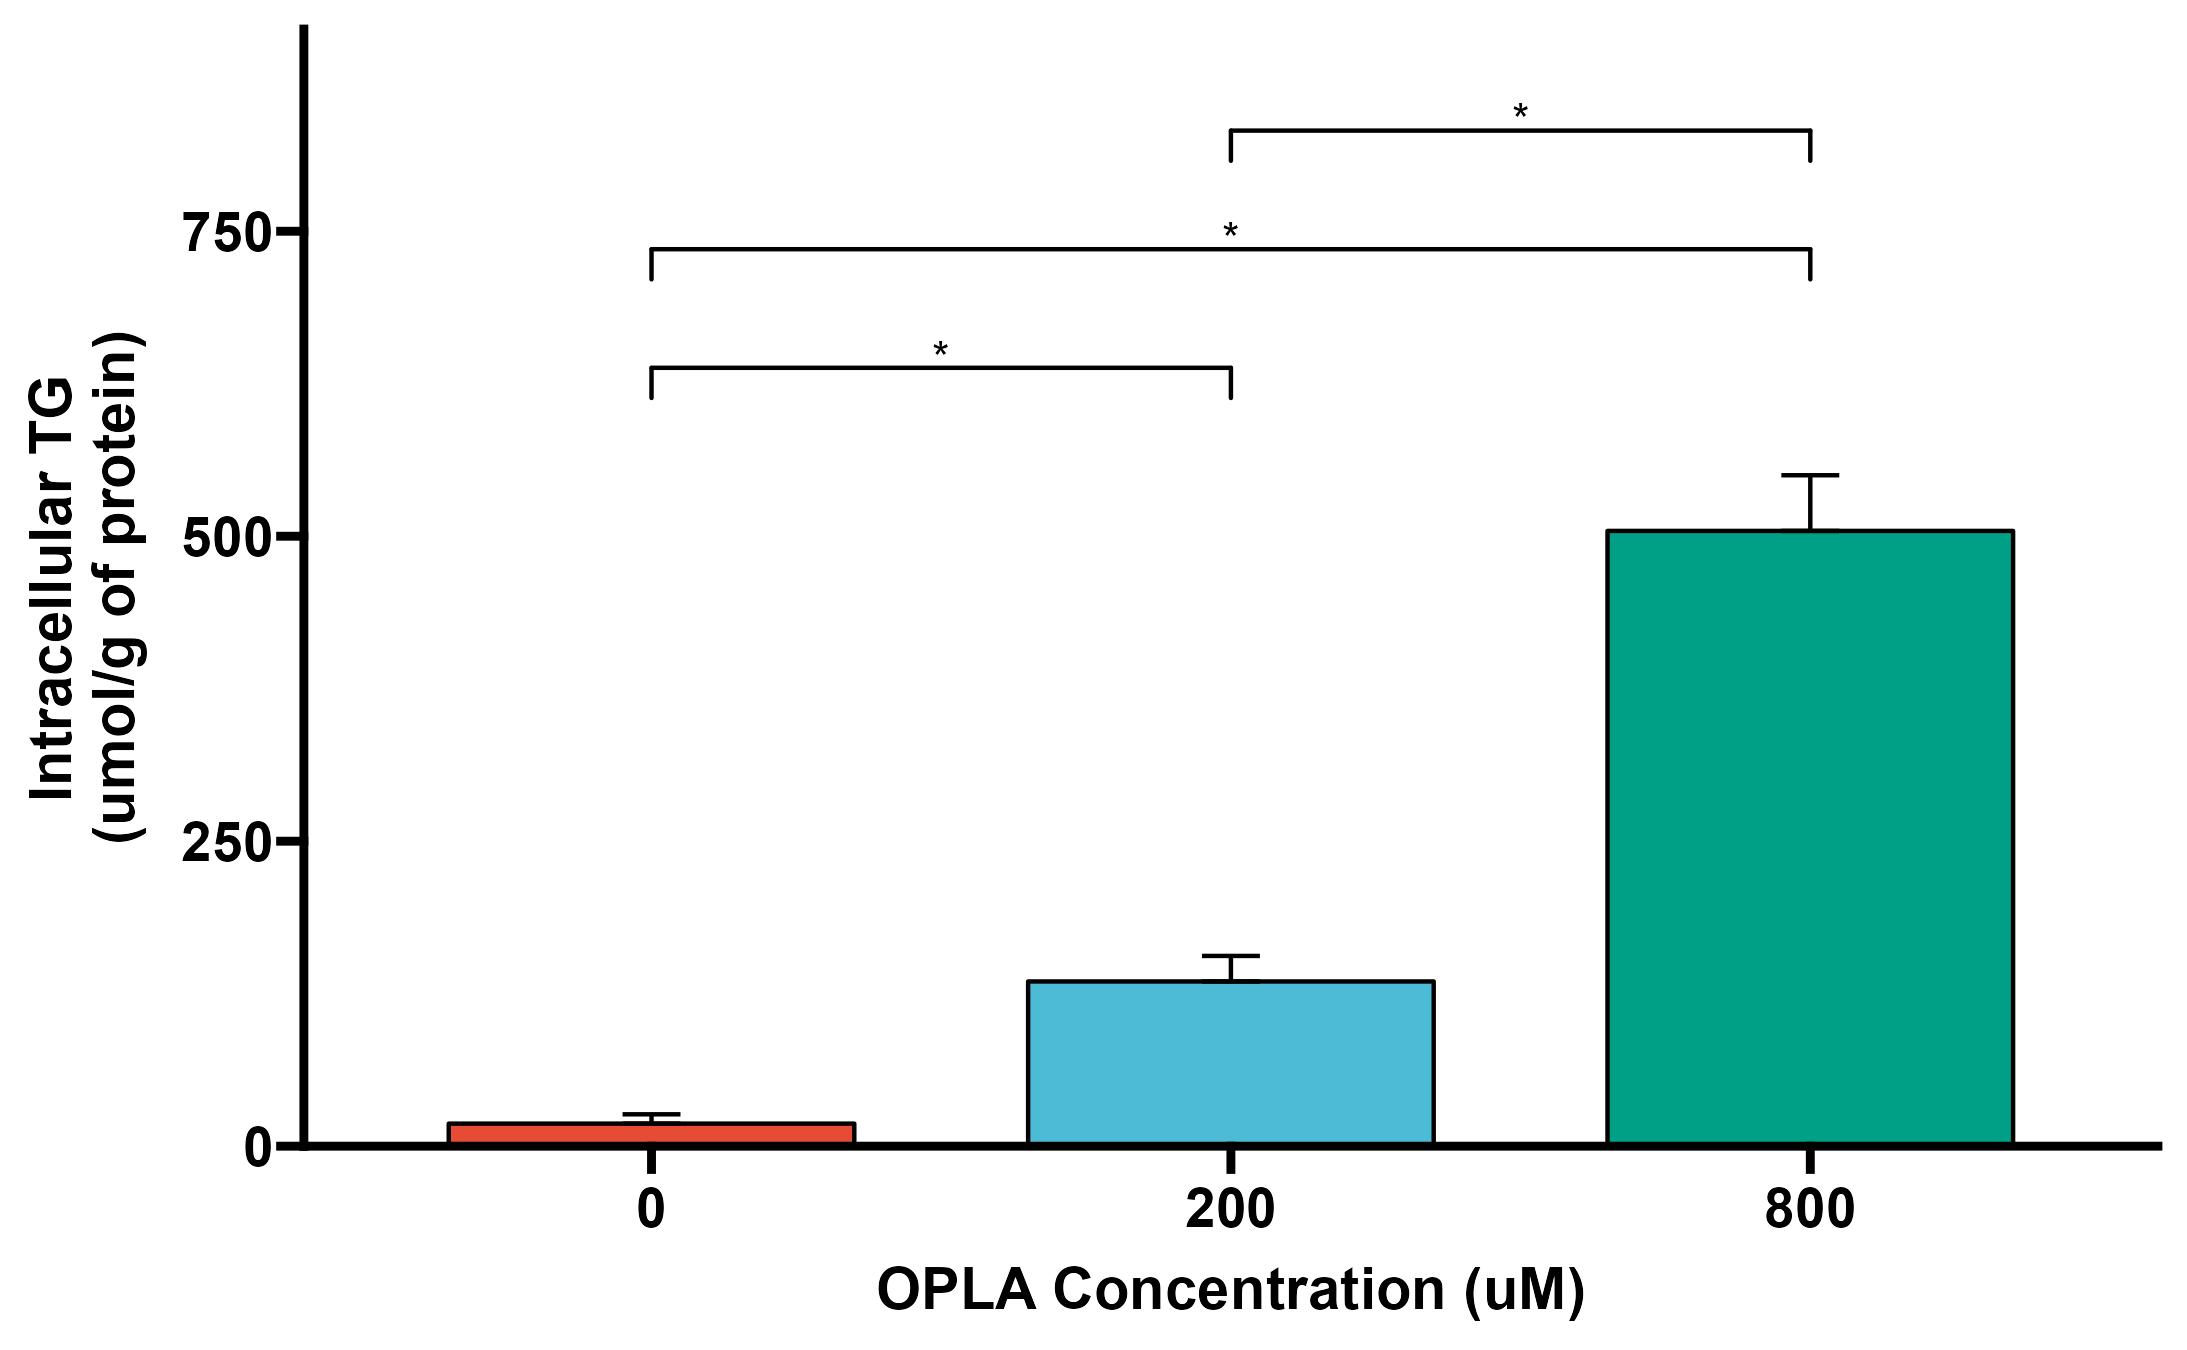
\includegraphics[width=0.49\textwidth]{figures/ch3-Model Development/LFHF TG.png}};
  \tikz\node[inner sep=0pt,label={[anchor=north west]north west:\subref{fig:LFHF ATG genes}}] {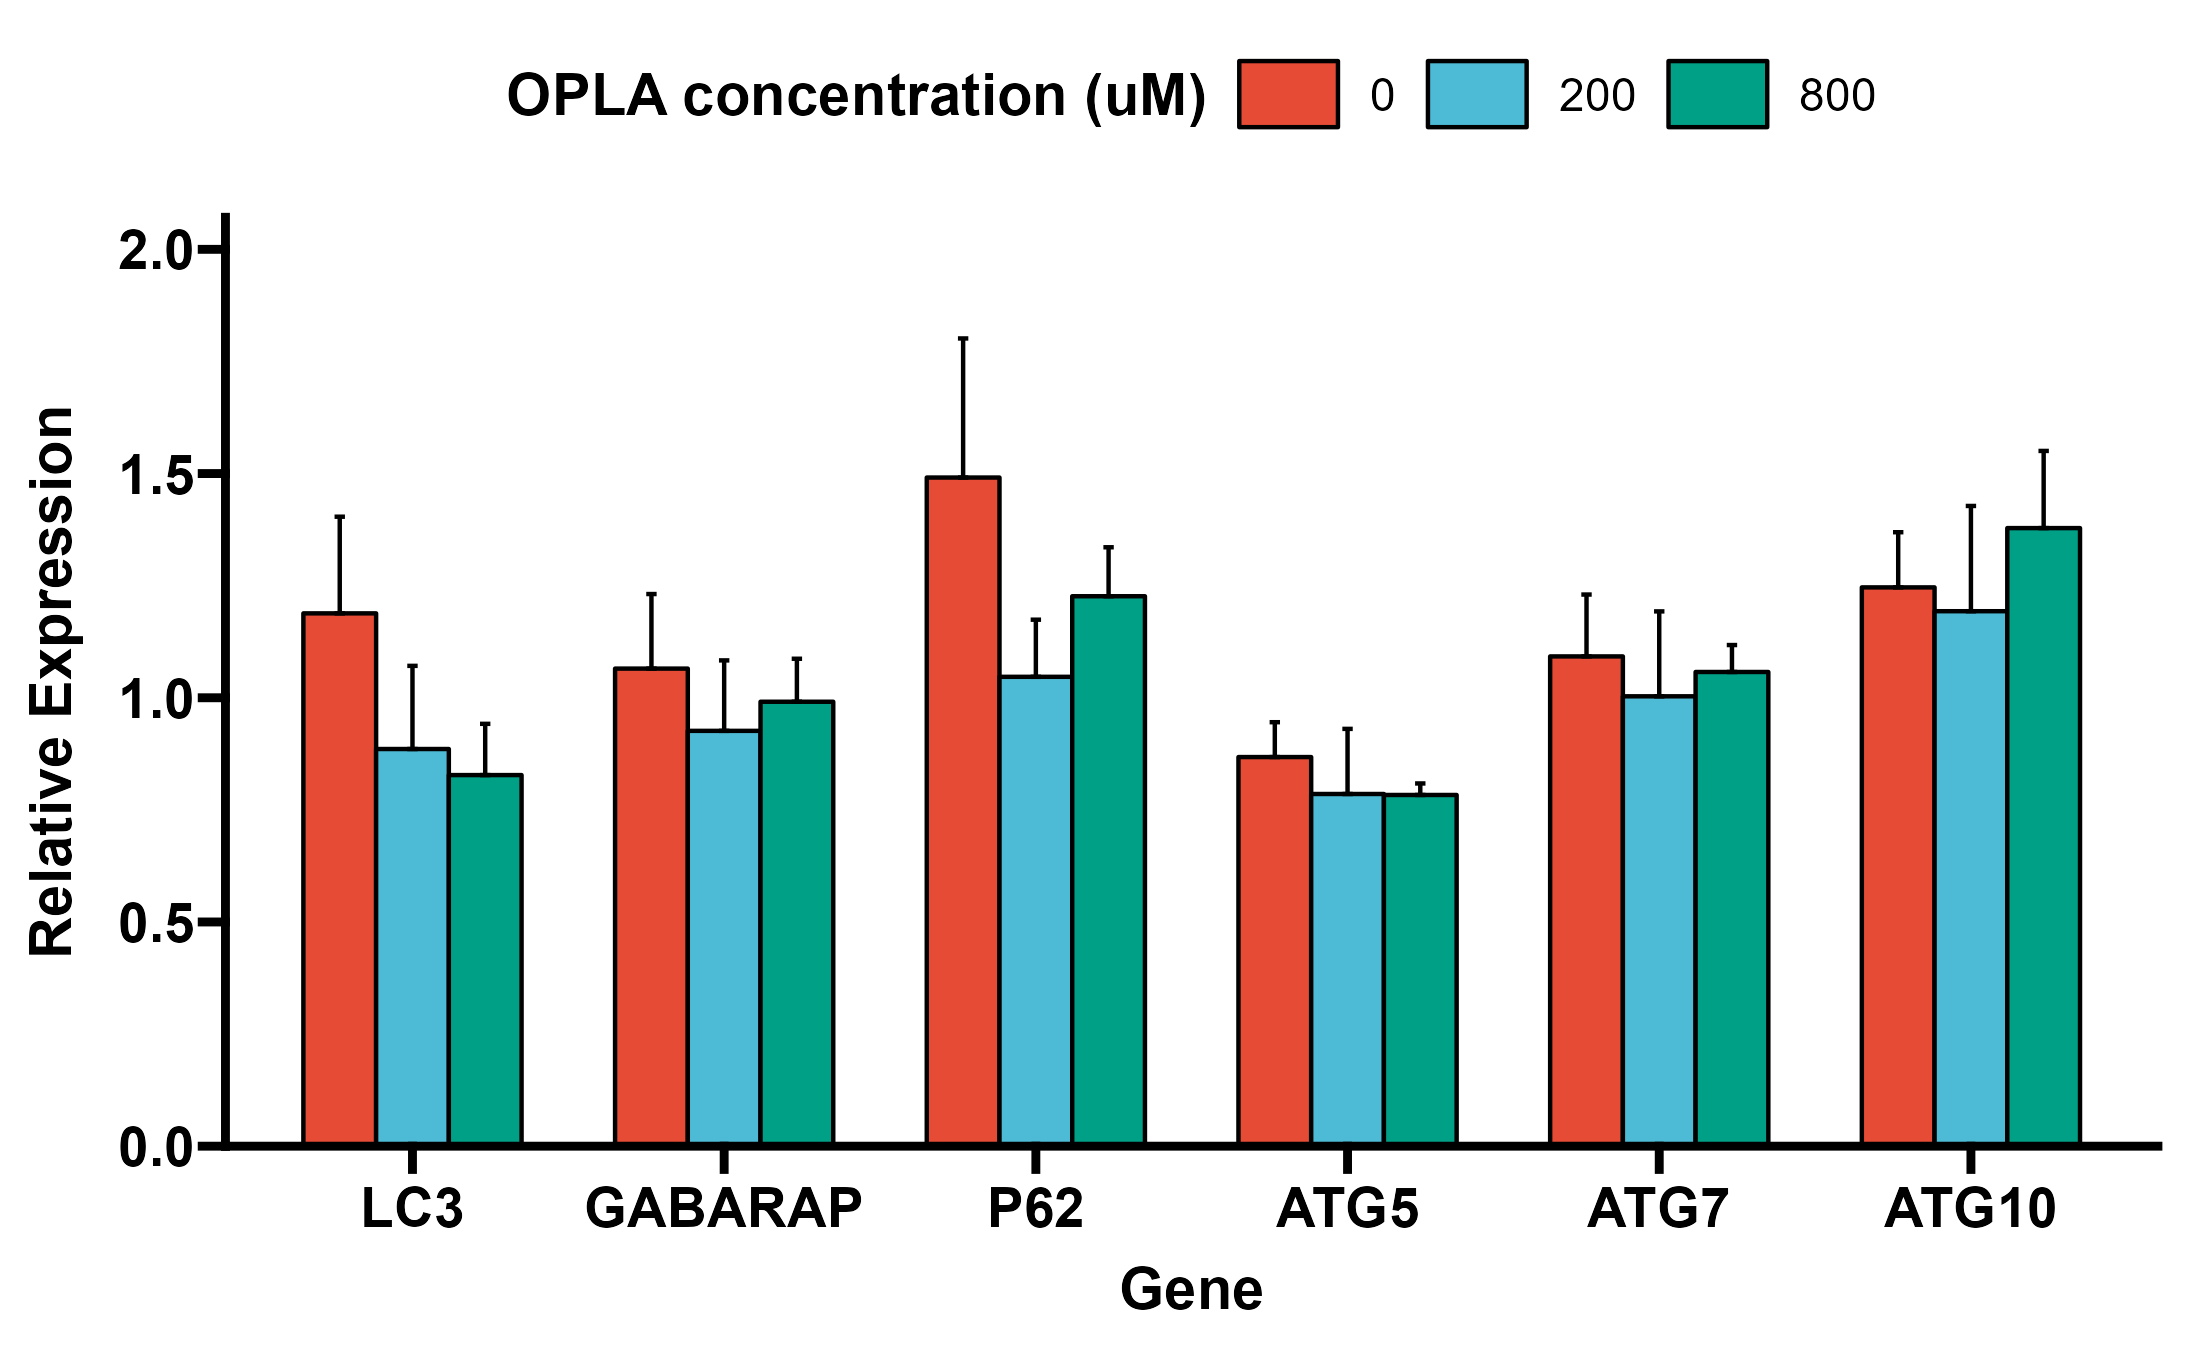
\includegraphics[width=0.49\textwidth]{figures/ch3-Model Development/LFHF ATG genes.png}};
   \tikz\node[inner sep=0pt,label={[anchor=north west]north west:\subref{fig:OPLA 0uM Picture}}] {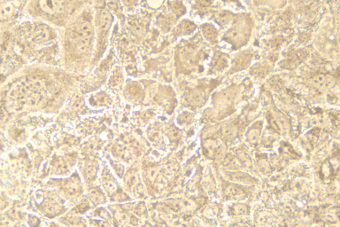
\includegraphics[width=0.49\textwidth]{figures/ch3-Model Development/OPLA 0uM Picture.png}};
      \tikz\node[inner sep=0pt,label={[anchor=north west]north west:\subref{fig:OPLA 800uM Picture}}] {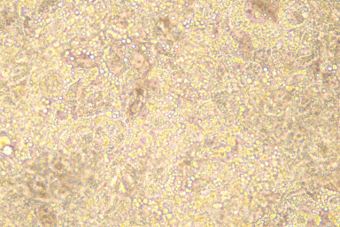
\includegraphics[width=0.49\textwidth]{figures/ch3-Model Development/OPLA 800uM Picture.png}};
    \caption{\textbf{Effect of media FA concentration on TG accumulation and autophagy.} Huh7 cells were cultured for 7 days in increasing concentrations of OPLA fatty acid mix. \textbf{A)} Lipids were extracted and intracellular TG content quantified by gas chromatography. \textbf{B)} RNA was extracted to measure autophagic gene expression relative to three housekeeper genes. Representative images (40x magnification) of cells cultured with \textbf{C)} no FA and in \textbf{D)} 800μM OPLA FA mix. Graphs representative of three biological repeats (n=3) carried out in technical triplicate. * p < 0.05. Abbreviations: TG, Triglyceride.}
            \label{fig:ch3-Model Development LFHF}
\end{figure}


\subsection{Effect of media FA composition on TG accumulation and autophagy}

Culturing Huh7 cells in predominantly unsaturated (OPLA) or saturated (POLA) FAs resulted in a similar increase in intracellular TG content, when compared to control media free from FAs (Figure \ref{fig:OPLAPOLA TG}). Intracellular TG composition reflected that of the FAs the cells were cultured in (Figure \ref{fig:OPLAPOLA Lipid}). Autophagic flux was then assessed by measuring LC3-II protein intensity (relative to housekeeper protein $\alpha$-Tubulin) with and without the autophagic inhibitor BAF. As LC3-II is normally degraded during autophagy, it's accumulation during autophagic inhibition is reflective of overall autophagic flux \cite{DJ2021Guidelines1}. There was no significant difference in autophagic flux between control, OPLA and POLA conditions, though there was a trend towards a decrease in cells treated with FAs (Figures \ref{fig:OPLAPOLA ATG FLX} - \ref{fig:OPLAPOLA WB Photo}).

\begin{figure}[h!]
  \centering
  {\phantomsubcaption\label{fig:OPLAPOLA TG}}
  {\phantomsubcaption\label{fig:OPLAPOLA Lipid}}
   {\phantomsubcaption\label{fig:OPLAPOLA ATG FLX}}
    {\phantomsubcaption\label{fig:OPLAPOLA BAF}}
     {\phantomsubcaption\label{fig:OPLAPOLA WB Photo}}
  \tikz\node[inner sep=0pt,label={[anchor=north west]north west:\subref{fig:OPLAPOLA TG}}] {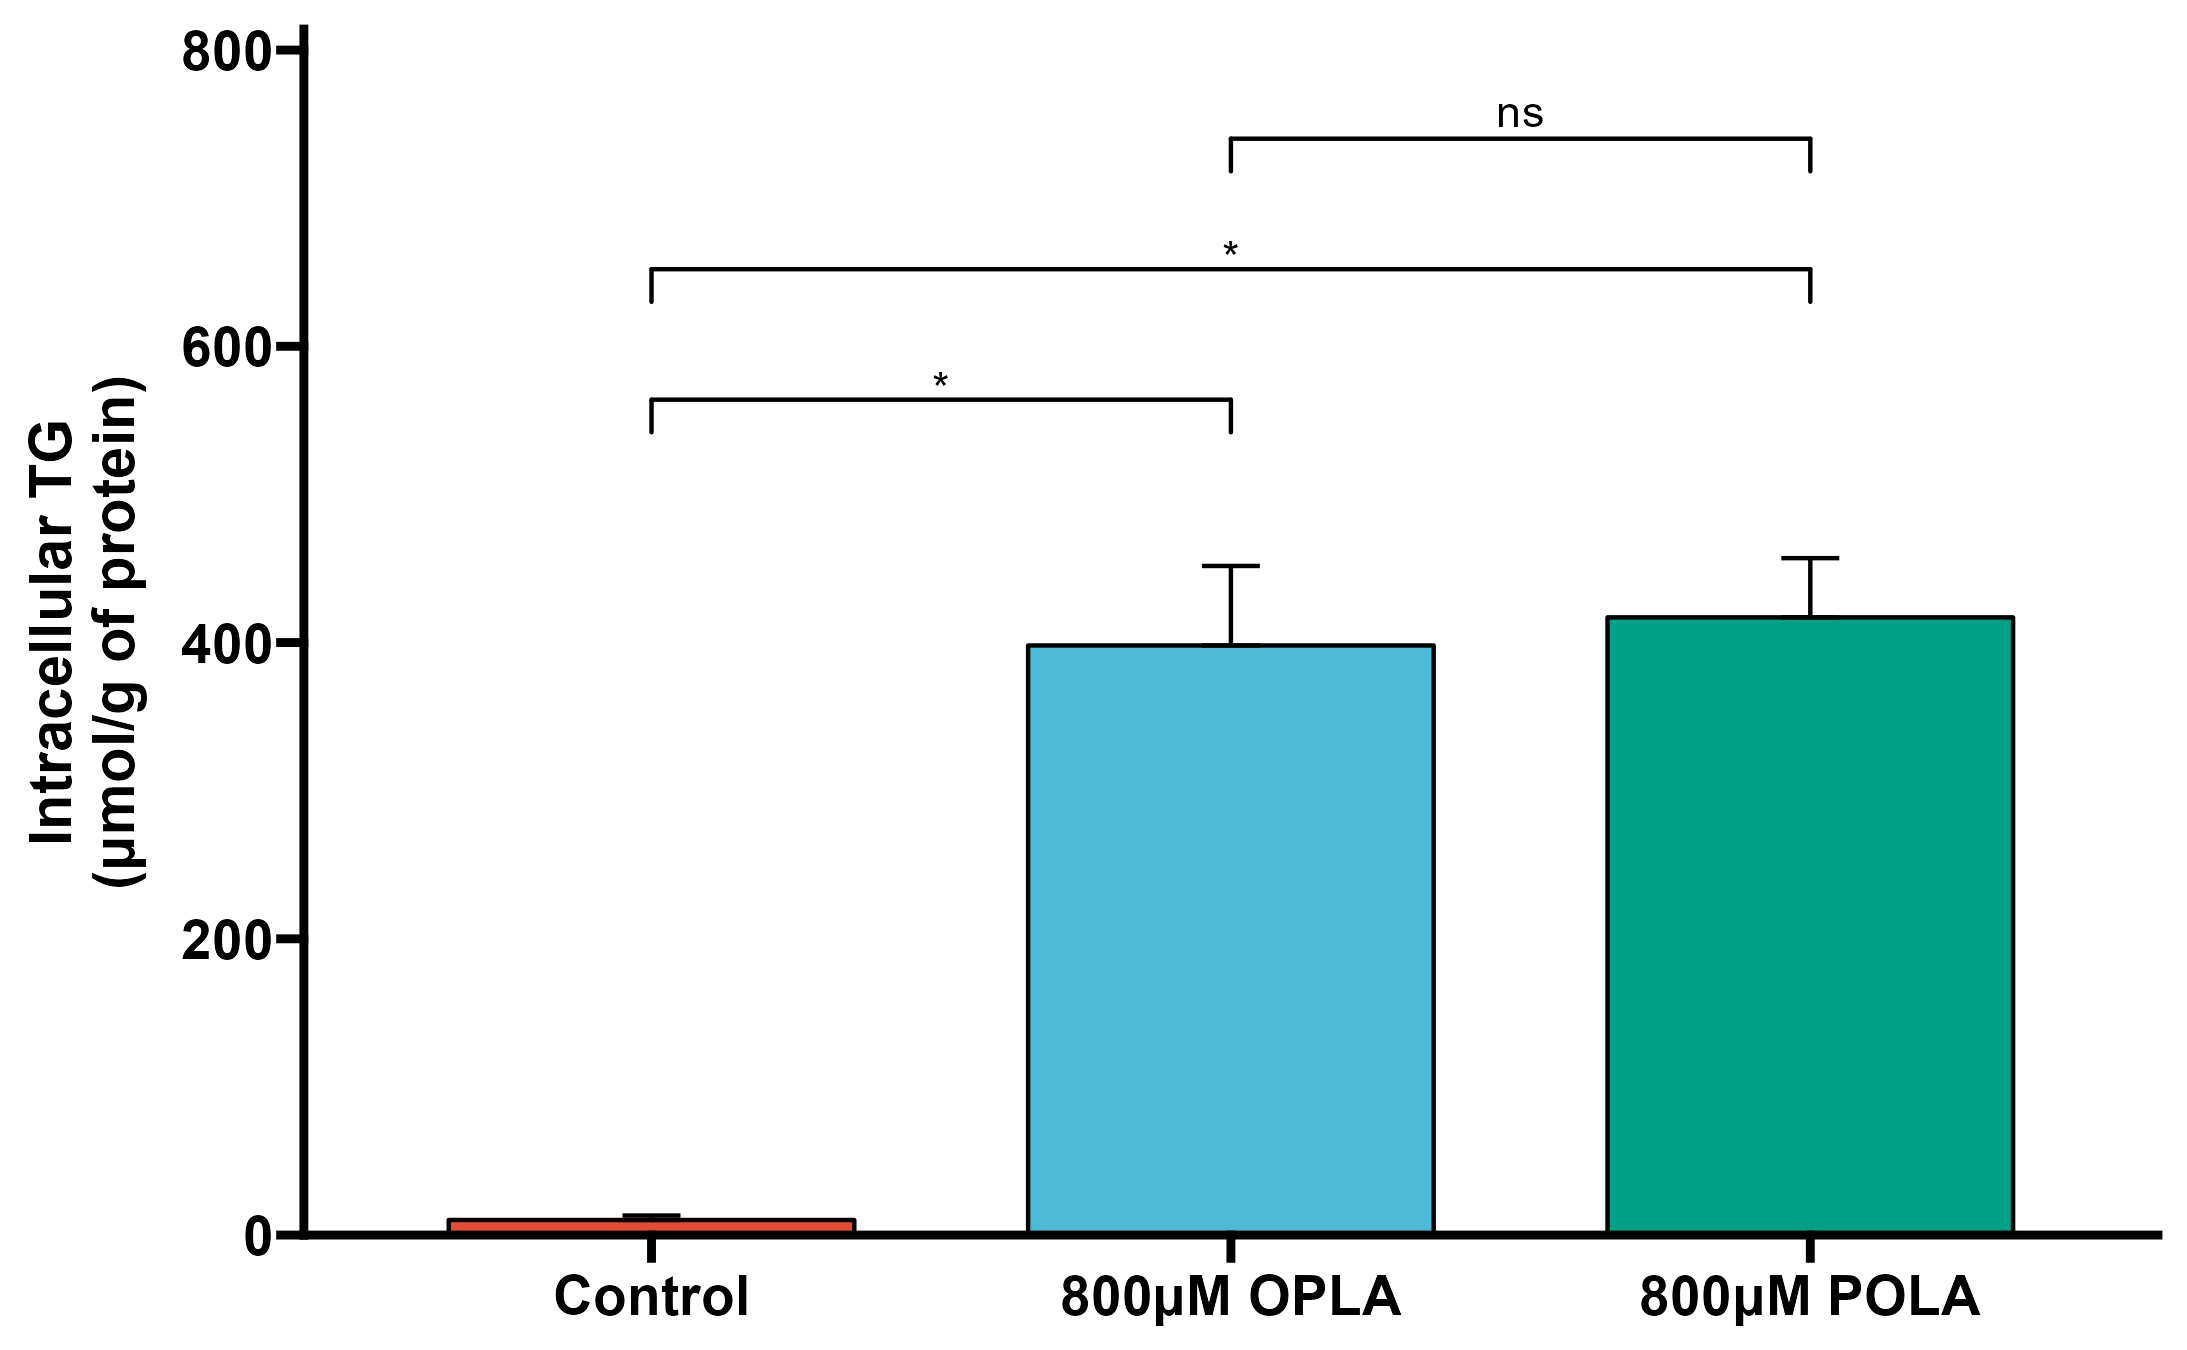
\includegraphics[width=0.49\textwidth]{figures/ch3-Model Development/OPLAPOLA TG.png}};
  \tikz\node[inner sep=0pt,label={[anchor=north west]north west:\subref{fig:OPLAPOLA Lipid}}] {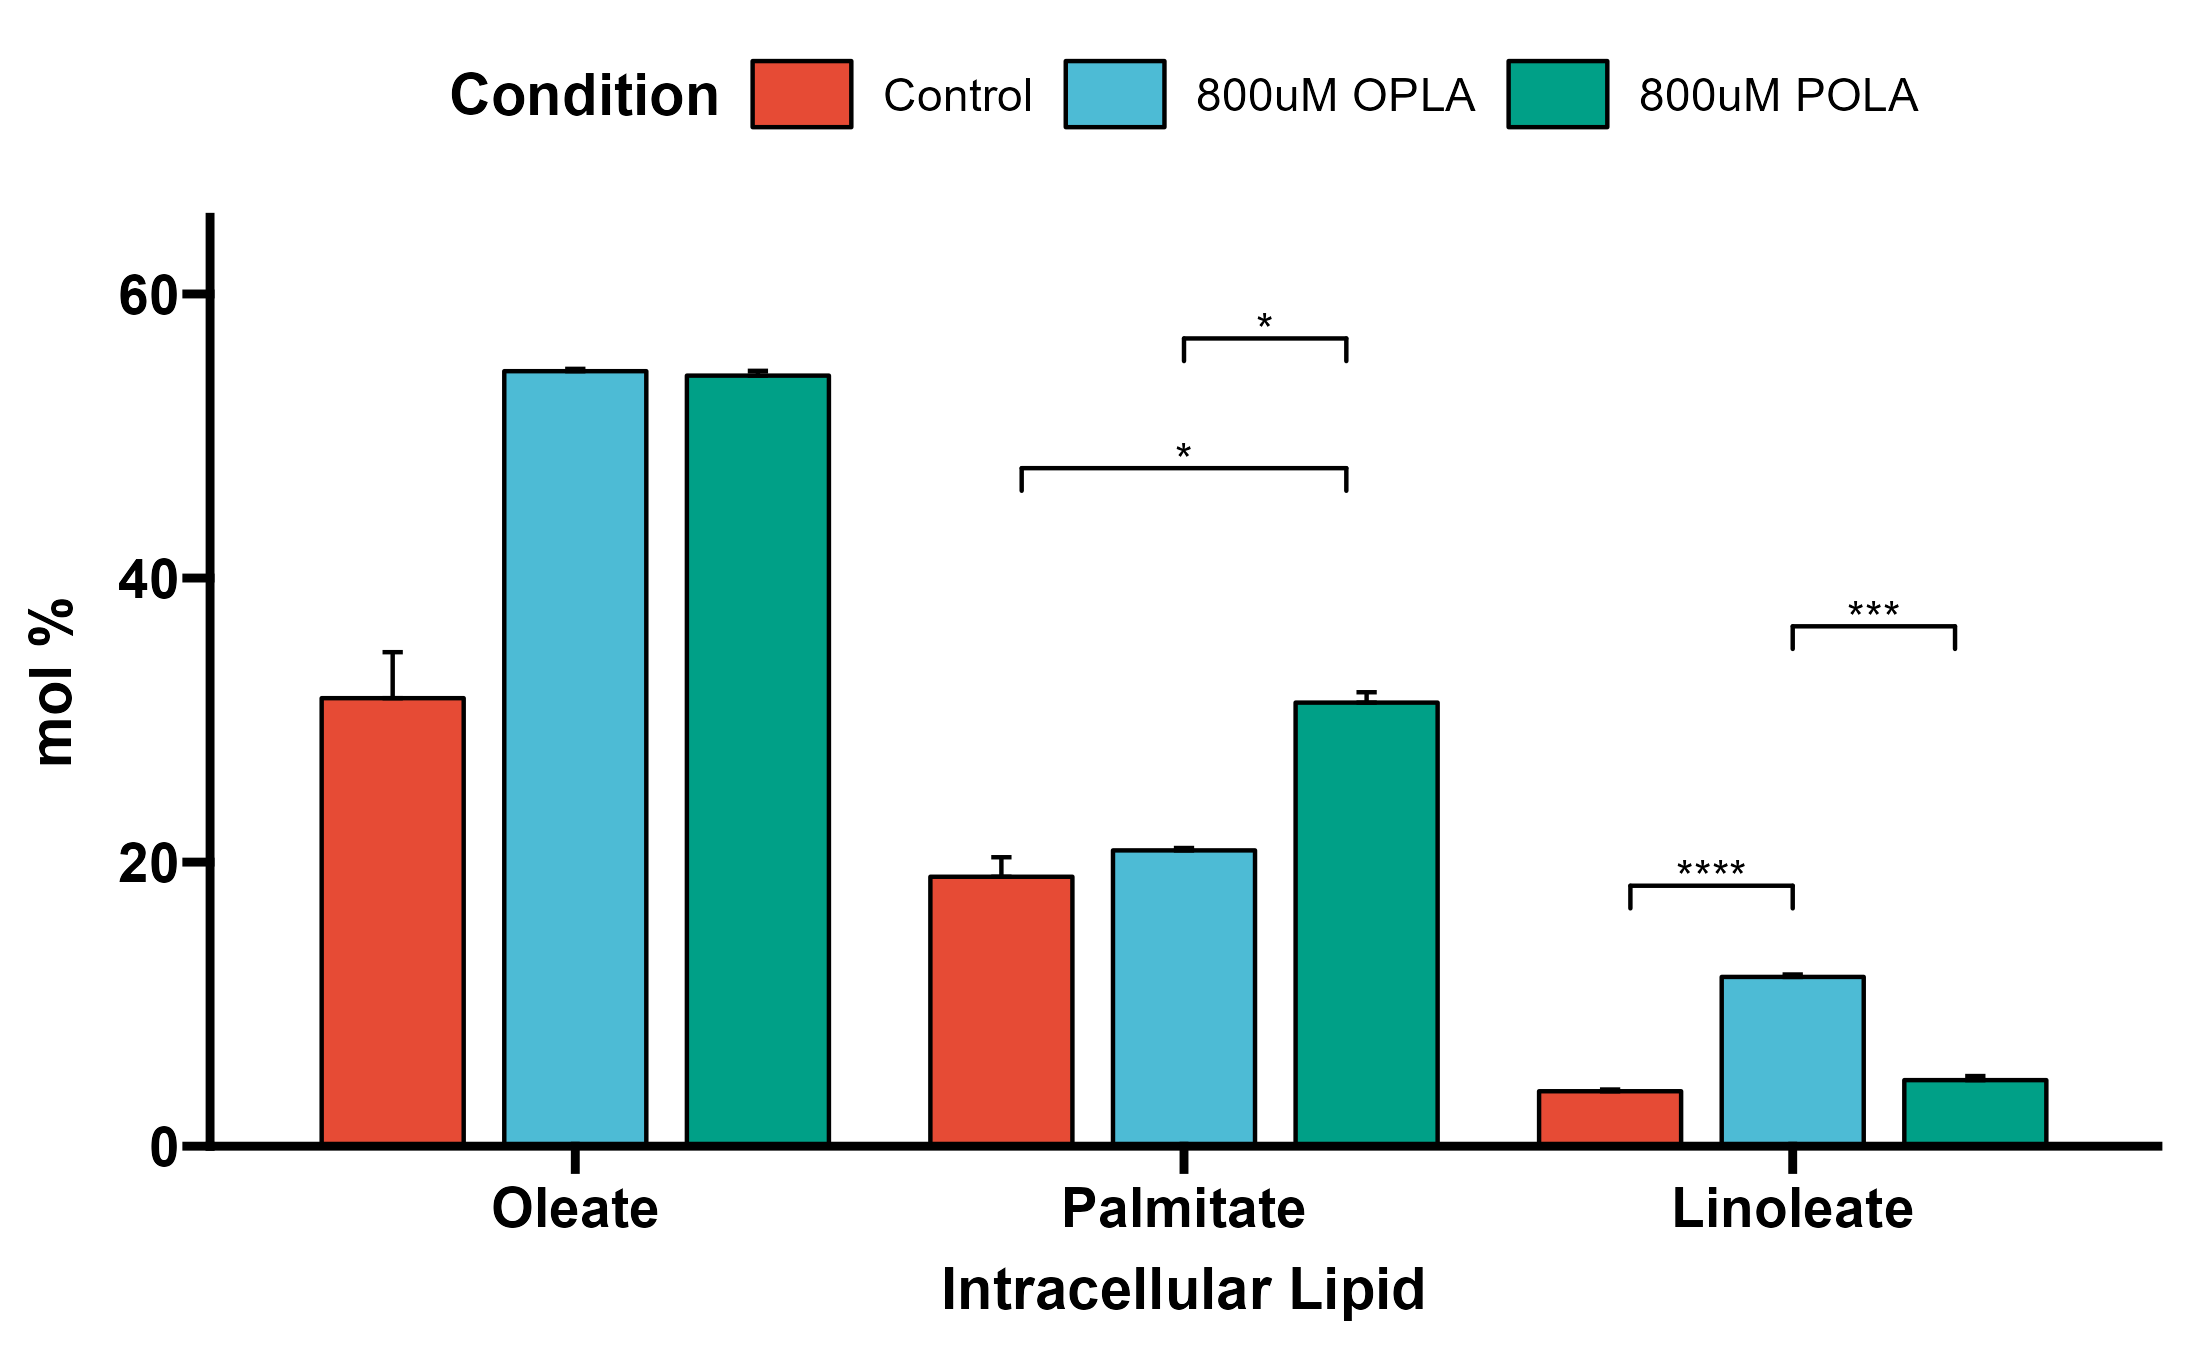
\includegraphics[width=0.49\textwidth]{figures/ch3-Model Development/OPLAPOLA Lipid contributions.png}};
   \tikz\node[inner sep=0pt,label={[anchor=north west]north west:\subref{fig:OPLAPOLA ATG FLX}}] {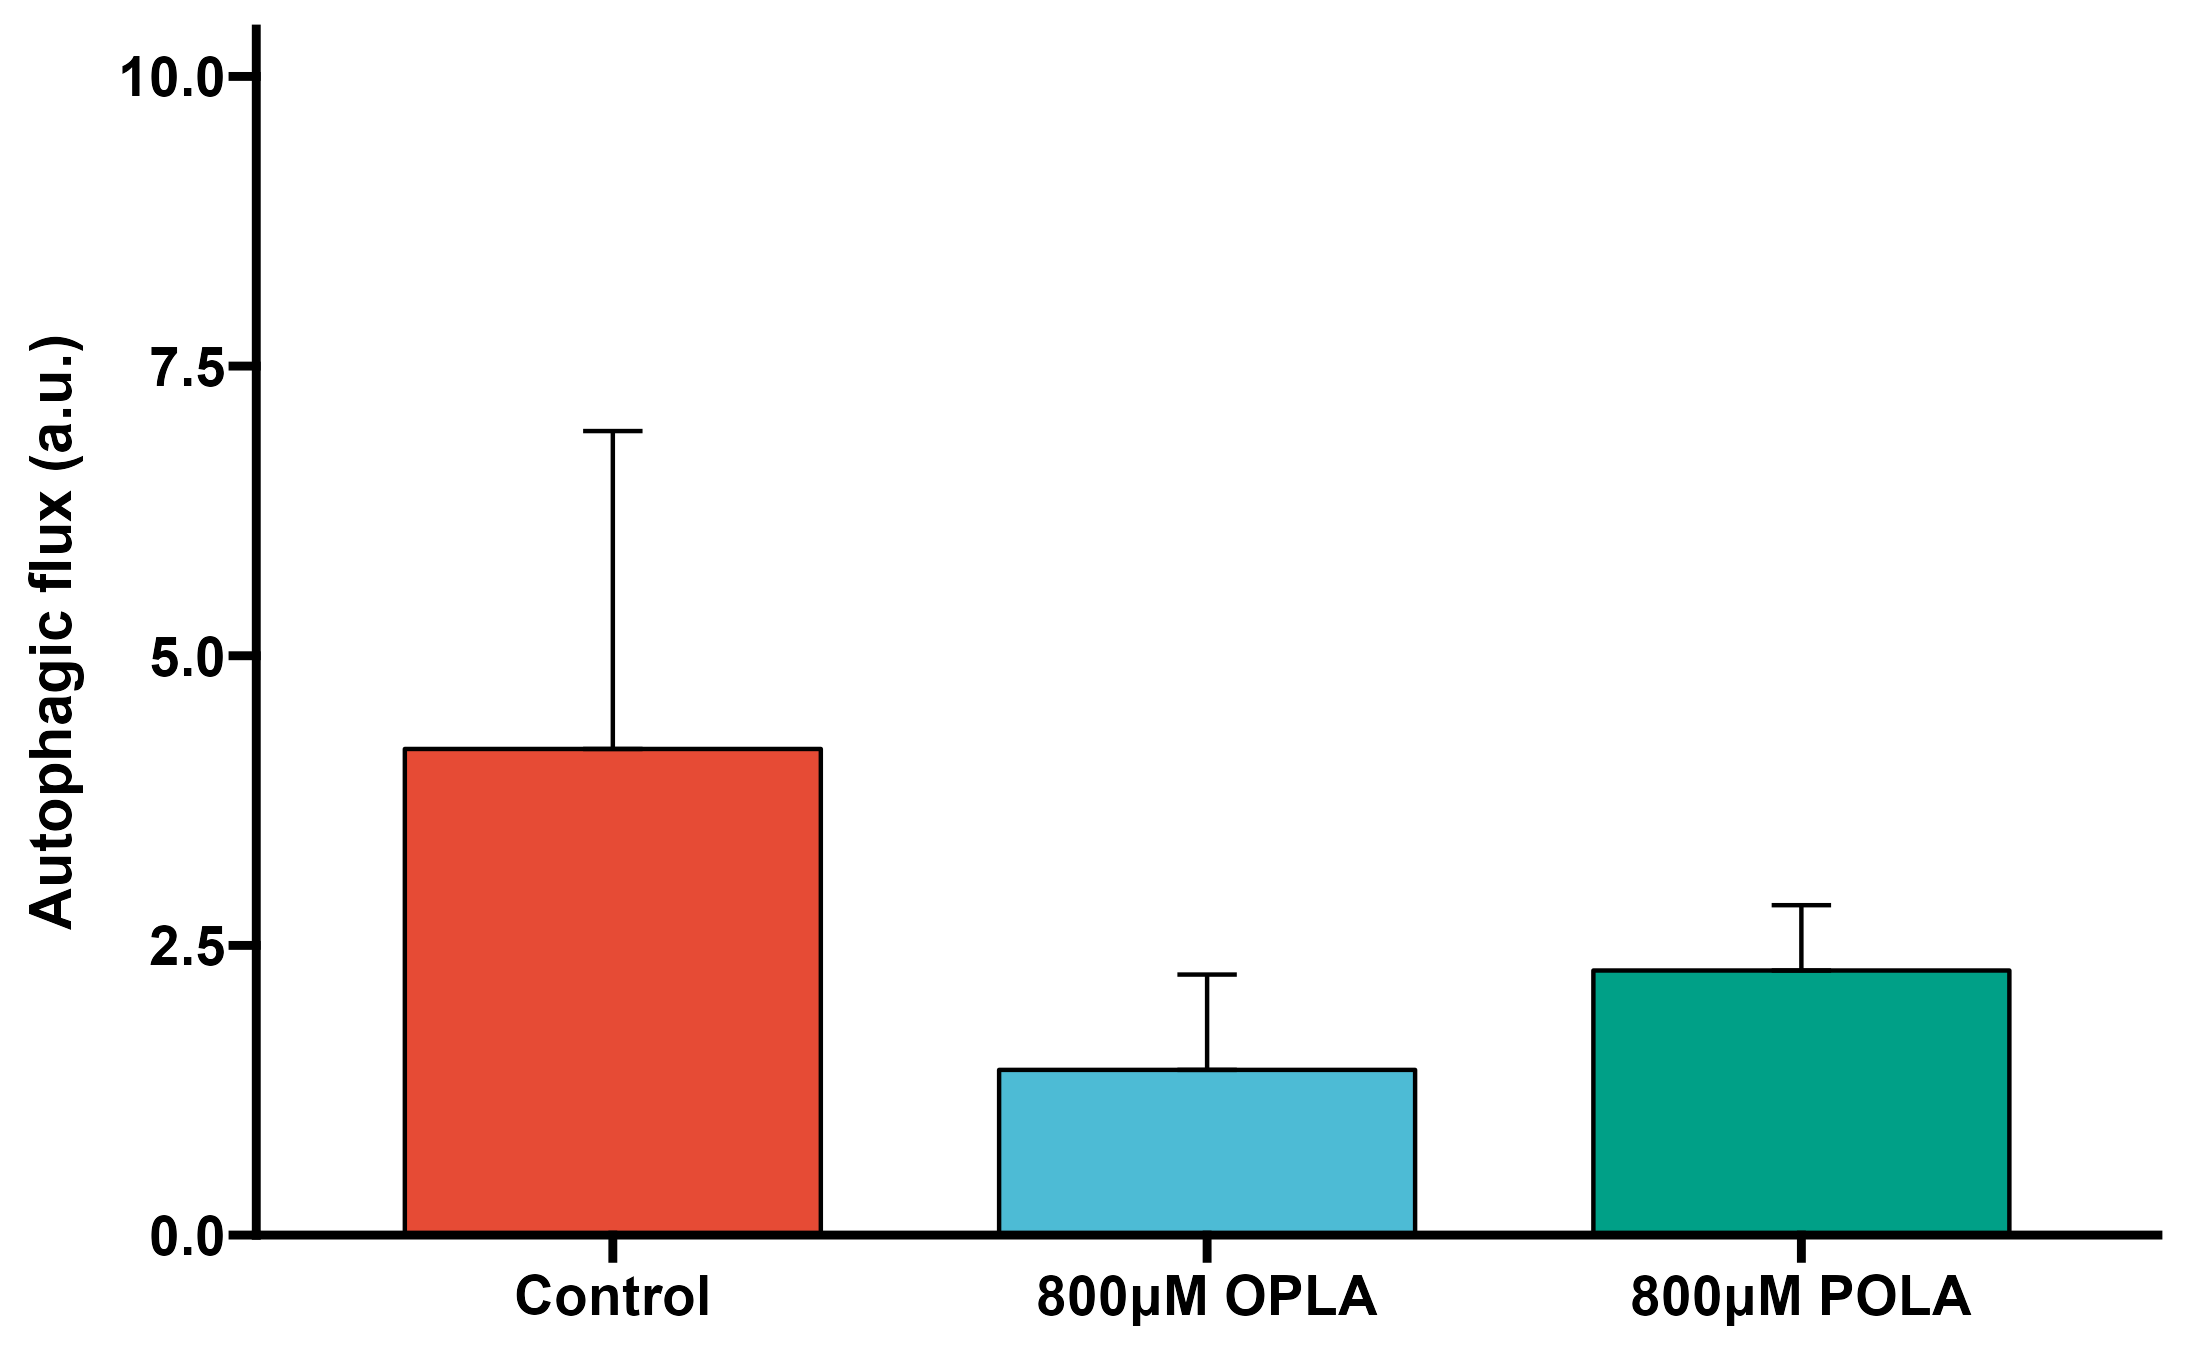
\includegraphics[width=0.49\textwidth]{figures/ch3-Model Development/OPLAPOLA ATG FLX.png}};
      \tikz\node[inner sep=0pt,label={[anchor=north west]north west:\subref{fig:OPLAPOLA BAF}}] {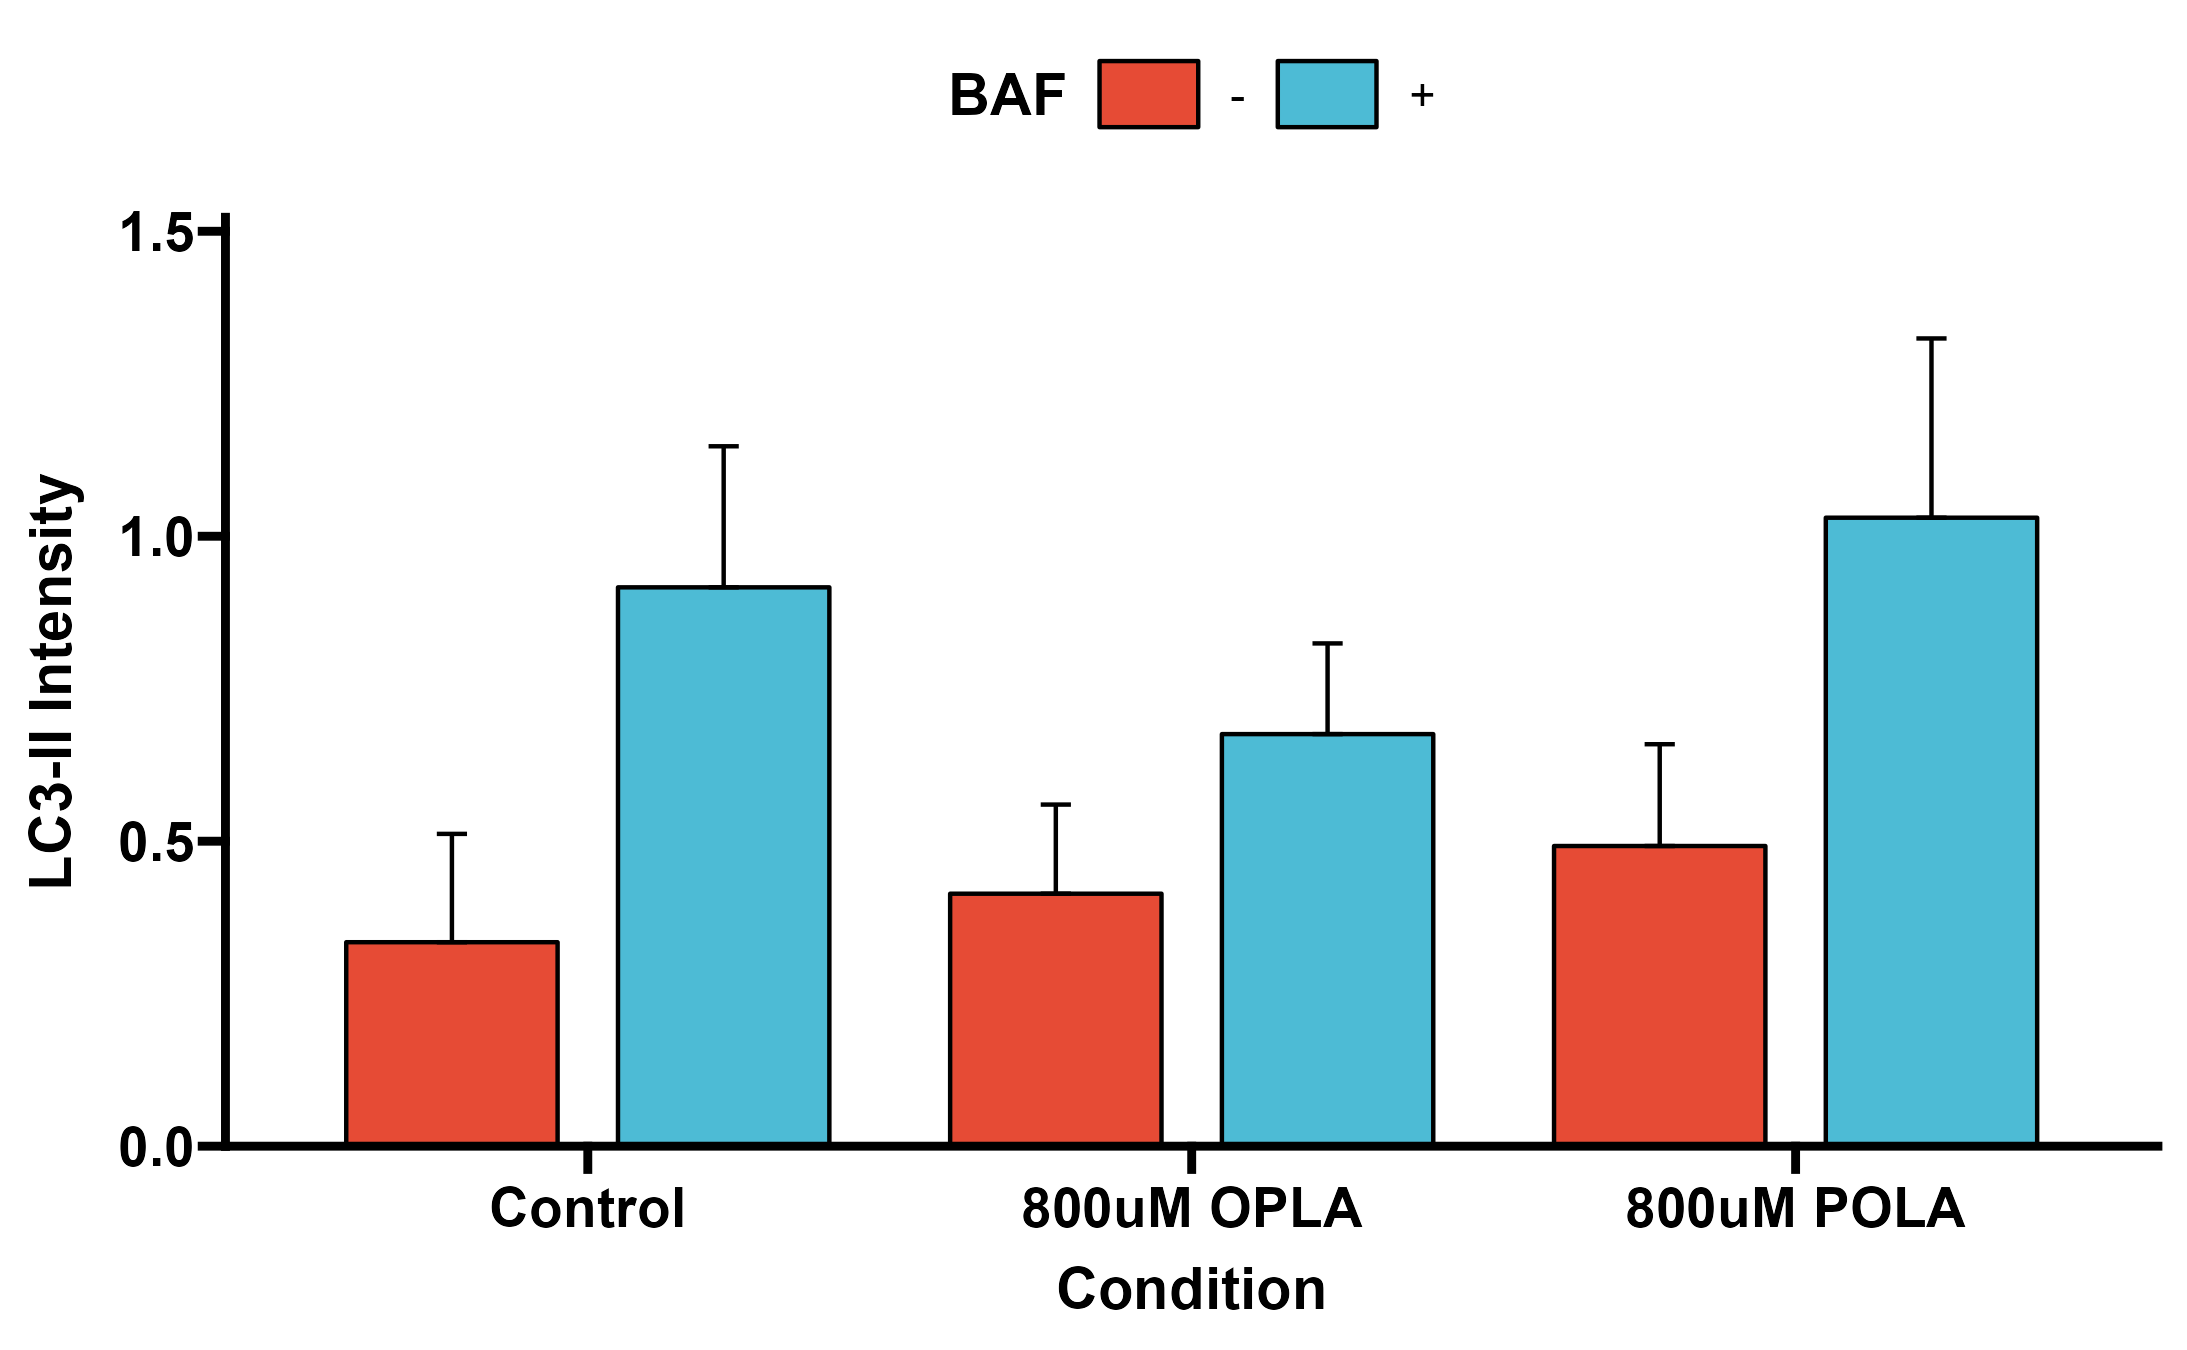
\includegraphics[width=0.49\textwidth]{figures/ch3-Model Development/OPLAPOLA BAF.png}};
      \tikz\node[inner sep=0pt,label={[anchor=north west]north west:\subref{fig:OPLAPOLA WB Photo}}] {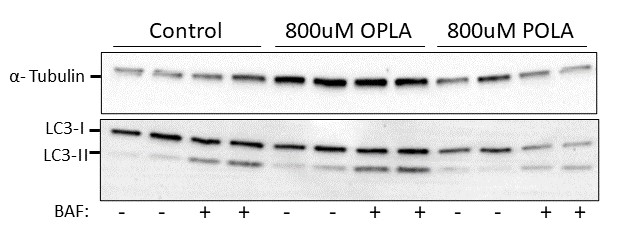
\includegraphics[width=0.6\textwidth]{figures/ch3-Model Development/OPLAPOLA WB Photo.jpg}};
        \caption{\textbf{Effect of media FA composition on TG accumulation and autophagy.} Cells were cultured for 7 days in either media with no FA (Control), a predominantly unsaturated FA mix (OPLA) or a predominantly saturated FA mix (POLA). Lipids were extracted and quantified by gas chromatography to measure \textbf{A)} total intracellular TG and \textbf{B)} the composition of intracellular TG. \textbf{C-E)} Autophagic flux was calculated as LC3-II intensity (relative to housekeeper protein $\alpha$-Tubulin): (BAF - Basal)/Basal. Representative of three biological repeats (n=3) carried out in technical duplicate. * p < 0.05, ** p < 0.01, *** p < 0.001. Abbreviations: BAF, Bafilomycin A1; TG, Triglyceride.}
        \label{fig:OPLAPOLA}
\end{figure}


%% APPENDICES %% 
% Starts lettered appendices, adds a heading in table of contents, and adds a
%    page that just says "Appendices" to signal the end of your main text.
\startappendices
% Add or remove any appendices you'd like here:

\chapter{\label{app:1-cardiophys}Review of Cardiac Physiology and Electrophysiology}

\minitoc

Appendices are just like chapters.  Their sections and subsections get numbered and included in the table of contents; figures and equations and tables added up, etc.  Lorem ipsum dolor sit amet, consectetur adipiscing elit. Sed et dui sem. Aliquam dictum et ante ut semper. Donec sollicitudin sed quam at aliquet. Sed maximus diam elementum justo auctor, eget volutpat elit eleifend. Curabitur hendrerit ligula in erat feugiat, at rutrum risus suscipit. Pellentesque habitant morbi tristique senectus et netus et malesuada fames ac turpis egestas. Integer risus nulla, facilisis eget lacinia a, pretium mattis metus. Vestibulum aliquam varius ligula nec consectetur. Maecenas ac ipsum odio. Cras ac elit consequat, eleifend ipsum sodales, euismod nunc. Nam vitae tempor enim, sit amet eleifend nisi. Etiam at erat vel neque consequat.

\section{Anatomy}
\label{sec:anatomy}

Lorem ipsum dolor sit amet, consectetur adipiscing elit. Donec accumsan cursus neque. Pellentesque eget tempor turpis, quis malesuada dui. Proin egestas, sapien sit amet feugiat vulputate, nunc nibh mollis nunc, nec auctor turpis purus sed metus. Aenean consequat leo congue volutpat euismod. Vestibulum et vulputate nisl, at ultrices ligula. Cras pulvinar lacinia ipsum at bibendum. In ac augue ut ante mollis molestie in a arcu.

Etiam vitae quam sollicitudin, luctus tortor eu, efficitur nunc. Vestibulum maximus, ante quis consequat sagittis, augue velit luctus odio, in scelerisque arcu magna id diam. Proin et mauris congue magna auctor pretium id sit amet felis. Maecenas sit amet lorem ipsum. Proin a risus diam. Integer tempus eget est condimentum faucibus. Suspendisse sem metus, consequat vel ante eget, porttitor maximus dui. Nunc dapibus tincidunt enim, non aliquam diam vehicula sed. Proin vel felis ut quam porta tempor. Vestibulum elit mi, dictum eget augue non, volutpat imperdiet eros. Praesent ac egestas neque, et vehicula felis.

Pellentesque malesuada volutpat justo, id eleifend leo pharetra at. Pellentesque feugiat rutrum lobortis. Curabitur hendrerit erat porta massa tincidunt rutrum. Donec tincidunt facilisis luctus. Aliquam dapibus sodales consectetur. Suspendisse lacinia, ipsum sit amet elementum fermentum, nulla urna mattis erat, eu porta metus ipsum vel purus. Fusce eget sem nisl. Pellentesque dapibus, urna vitae tristique aliquam, purus leo gravida nunc, id faucibus ipsum magna aliquet ligula. Lorem ipsum dolor sit amet, consectetur adipiscing elit. Proin sem lacus, rutrum eget efficitur sed, aliquam vel augue. Aliquam ut eros vitae sem cursus ultrices ut ornare urna. Nullam tempor porta enim, in pellentesque arcu commodo quis. Interdum et malesuada fames ac ante ipsum primis in faucibus. Curabitur maximus orci purus, ut molestie turpis pellentesque ut.

Donec lacinia tristique ultricies. Proin dignissim risus ut dolor pulvinar mollis. Proin ac turpis vitae nibh finibus ullamcorper viverra quis felis. Mauris pellentesque neque diam, id feugiat diam vestibulum vitae. In suscipit dui eu libero ultrices, et sagittis nunc blandit. Aliquam at aliquet ex. Nullam molestie pulvinar ex vitae interdum. Praesent purus nunc, gravida id est consectetur, convallis elementum nulla. Praesent ex dolor, maximus eu facilisis at, viverra eget nulla. Donec ullamcorper ante nisi. Sed volutpat diam eros. Nullam egestas neque non tortor aliquet, sed pretium velit tincidunt. Aenean condimentum, est ac vestibulum mattis, quam augue congue augue, mattis ultrices nibh libero non ante. Lorem ipsum dolor sit amet, consectetur adipiscing elit.

Aenean volutpat eros tortor, non convallis sapien blandit et. Maecenas faucibus nulla a magna posuere commodo. Nullam laoreet ante a turpis laoreet malesuada. Phasellus in varius sem. Vestibulum sagittis nibh sed tincidunt blandit. Donec aliquam accumsan odio sit amet lacinia. Integer in tellus diam. Vivamus varius massa leo, vitae ullamcorper metus pulvinar sed. Maecenas nec lorem ornare, elementum est quis, gravida massa. Suspendisse volutpat odio ex, ac ultrices leo ultrices vel. Sed sed convallis ipsum. Pellentesque euismod a nulla sed rhoncus. Sed vehicula urna vitae mi aliquet, non sodales lacus ullamcorper. Duis mattis justo turpis, id tempus est tempus eu. Curabitur vitae hendrerit ligula.

Curabitur non pretium enim, in commodo ligula. Etiam commodo eget ligula a lacinia. Vestibulum laoreet ante tellus, vel congue sapien ornare in. Donec venenatis cursus velit vitae pulvinar. Pellentesque habitant morbi tristique senectus et netus et malesuada fames ac turpis egestas. Suspendisse in metus lectus. Pellentesque gravida dolor eget finibus imperdiet. Duis id molestie tortor. Mauris laoreet faucibus facilisis. Aliquam vitae dictum massa, sit amet dignissim lacus.

Fusce eleifend tellus id ex consequat maximus. Donec ultrices ex ut turpis ornare, non molestie mi placerat. Nulla sit amet auctor nunc, sit amet euismod elit. Phasellus risus tellus, condimentum a metus et, venenatis tristique urna. Cras mattis felis eget ipsum fermentum egestas. Ut augue odio, venenatis id convallis vel, congue quis augue. Maecenas sed maximus est, posuere aliquet tortor. Ut condimentum egestas nisi eu porttitor. Ut mi turpis, posuere id lorem vel, elementum tempor arcu.

Morbi nisl arcu, venenatis non metus ac, ullamcorper scelerisque justo. Nulla et accumsan lorem. Mauris aliquet dui sit amet libero aliquet, in ornare metus porttitor. Integer ultricies urna eu consequat ultrices. Maecenas a justo id purus ultricies posuere sed et quam. Cum sociis natoque penatibus et magnis dis parturient montes, nascetur ridiculus mus. Sed eleifend risus quis aliquet gravida. Nullam ac erat porta est bibendum dictum in a dolor. Nam eget turpis viverra, vulputate lectus eget, mattis ligula. Nam at tellus eget dui lobortis sodales et ut augue. In vestibulum diam eget mi cursus, ut tincidunt nulla pellentesque.

Aliquam erat volutpat. Sed ultrices massa id ex mattis bibendum. Nunc augue magna, ornare at aliquet gravida, vehicula sed lorem. Quisque lobortis ipsum eu posuere eleifend. Duis bibendum cursus viverra. Nam venenatis elit leo, vitae feugiat quam aliquet sed. Cras velit est, tempus ac lorem sed, pharetra lobortis ipsum. Donec suscipit gravida interdum. Nunc non finibus est. Nullam turpis elit, tempus non ante.

\section{Mechanical Cycle}

Lorem ipsum dolor sit amet, consectetur adipiscing elit. Aenean tellus est, suscipit sed facilisis quis, malesuada at ipsum. Nam tristique urna quis quam iaculis, et mattis orci pretium. Praesent euismod elit vel metus commodo ultrices. Vestibulum et tincidunt ex, in molestie ex. Donec ullamcorper sollicitudin accumsan. Etiam ac leo turpis. Duis a tortor felis. Nullam sollicitudin eu purus ac hendrerit. Nam hendrerit ligula libero, eget finibus orci bibendum a. Aenean ut ipsum magna.

Ut viverra, sapien sed accumsan blandit, nisi sem tempus tellus, at suscipit magna erat ornare nunc. Proin lacinia, nisi ut rutrum malesuada, nibh quam pellentesque nunc, sit amet consectetur purus felis ac tortor. Suspendisse lacinia ipsum eu sapien pellentesque mattis. Mauris ipsum nunc, placerat non diam vel, efficitur laoreet nunc. Sed lobortis, ipsum eget gravida facilisis, sem nulla viverra mi, in placerat eros sem viverra lacus. Aliquam porta aliquet diam vel commodo. Nulla facilisi. Duis erat libero, lobortis vel hendrerit vitae, sagittis id dui. Nulla pretium eros nec quam tincidunt, vel luctus mi aliquam. Integer imperdiet purus in est tristique venenatis. Ut pellentesque, nunc vitae iaculis ultricies, urna turpis dignissim risus, a laoreet felis magna nec erat.

Quisque sollicitudin faucibus ligula, et egestas nibh dictum sit amet. Proin eu mi a lectus congue pretium eu quis arcu. Suspendisse vehicula libero eu ipsum aliquam, vel elementum nibh mattis. Sed sed sapien vitae turpis tristique pulvinar a ut metus. Etiam semper gravida est, mollis gravida est porta ac. Proin eget tincidunt erat. Maecenas ultrices erat eget purus ultricies, ut lacinia arcu dictum. Nam et nisi sit amet ex congue mattis vel eget lorem. Aliquam erat volutpat. Pellentesque porttitor nibh vitae elementum consectetur. Aenean et est lobortis, congue sapien non, ullamcorper sapien. Ut facilisis sem non dapibus vehicula.

Mauris euismod odio dolor, sit amet gravida mauris placerat et. Curabitur nec dolor non nibh molestie lobortis dignissim non ante. Nullam rutrum lobortis ultrices. Aenean ex erat, elementum sed maximus id, posuere id quam. Proin rutrum ex elit, pretium aliquam risus finibus at. Aenean egestas orci velit, sed aliquet sapien condimentum a. Duis consequat, arcu eu viverra venenatis, dolor lorem gravida lectus, non aliquet nisi sem at augue. Donec laoreet blandit luctus. Aenean vehicula nisl vel faucibus luctus. Sed ut semper velit, vitae laoreet magna. Sed at interdum magna.

Sed iaculis faucibus odio, eu aliquam purus efficitur vel. Cras at nulla ac enim congue varius ut et nulla. Integer blandit mattis augue.

\section{Electrical Cycle}
\label{sec:electcycle}

Lorem ipsum dolor sit amet, consectetur adipiscing elit. In faucibus condimentum rhoncus. Ut dictum nisl id risus gravida lobortis. Sed vehicula mollis tellus ut varius. Fusce eget egestas dui, et commodo dui. Proin sollicitudin interdum tempus. Nullam in elit a enim fringilla bibendum. Vestibulum sodales pellentesque condimentum. Nulla facilisi. Nunc et dolor in nulla eleifend dictum at vel ligula. Aliquam ut velit non elit ullamcorper porta ac et ex. Fusce ornare magna non nunc vestibulum, eget molestie quam dictum. In interdum aliquam odio, in posuere tellus convallis quis. Curabitur non diam elit. Proin vulputate orci diam, a tincidunt ante luctus eu. Ut a viverra ligula. Curabitur pulvinar tempus tellus eget suscipit.

Aliquam posuere massa at ante dapibus congue. Curabitur ullamcorper tortor eget consectetur aliquet. Mauris tempor magna id mauris fringilla, a varius erat blandit. Nam eleifend ullamcorper placerat. Phasellus augue tortor, volutpat bibendum lorem nec, fringilla volutpat nisl. Mauris cursus urna metus, vel eleifend orci iaculis ut. Sed sit amet scelerisque massa, quis consequat dui. Donec semper sem dui, ac placerat velit egestas vel. Nulla facilisi. Quisque tellus eros, sagittis malesuada augue ut, faucibus dictum nulla. Vestibulum non dapibus erat, ut consequat libero. Ut turpis mi, dapibus commodo libero lobortis, maximus vestibulum lectus. Vestibulum sit amet sapien dapibus, tincidunt leo in, suscipit arcu. Sed in erat bibendum, laoreet eros eu, pellentesque justo. Nulla sodales purus neque, eget maximus ipsum consequat at. Maecenas a nisl sagittis, tempus ipsum sed, dictum mauris.

Suspendisse posuere odio lacus, at auctor tortor vehicula sed. Phasellus suscipit ornare enim vitae placerat. Sed viverra purus vel sapien tempor, quis iaculis erat laoreet. Aenean vel nunc vestibulum, ornare nunc ac, mollis urna. Aenean ultrices felis ipsum, ac semper est ullamcorper in. Donec in justo varius, egestas tortor ut, venenatis augue. Duis mattis, ligula quis lacinia fringilla, tellus neque accumsan ipsum, vitae tempor metus elit vel nibh. Curabitur porttitor urna nec sapien tempor, et porttitor velit malesuada.

Suspendisse aliquam nisl quis placerat vulputate. Proin dapibus ipsum ac ante sagittis, volutpat auctor sem dapibus. Nam in facilisis odio. Integer ante mauris, eleifend et pulvinar in, venenatis quis ligula. Phasellus posuere sollicitudin tortor eget euismod. Maecenas mollis tortor eget justo vulputate sagittis. Etiam hendrerit massa quis ex molestie sodales. Quisque facilisis erat lacus, id convallis sem suscipit bibendum. Integer dui urna, pharetra sed porta sed, bibendum ut odio. Donec placerat at lectus egestas consequat. Sed id rhoncus est, vitae vulputate sapien. Fusce tempus quam lorem, id ornare turpis sodales sed. Integer aliquet urna eget condimentum consequat. Vestibulum quis dui vel ligula posuere luctus id nec turpis.

Nam vitae placerat lacus. Mauris scelerisque interdum volutpat. Nunc aliquet tristique enim, sit amet molestie felis ullamcorper vitae. Nullam sollicitudin orci orci, in condimentum tellus consectetur in. Nam id justo justo. Fusce eget finibus est. Proin id tortor nec quam cursus vehicula. Aliquam ultrices eros eros, a tincidunt elit eleifend auctor.

Nullam consectetur dapibus ligula sit amet efficitur. Nunc non posuere sapien. Vivamus dui nisl, aliquam id ipsum non, pulvinar ornare neque. Nunc rhoncus pretium congue. Fusce id laoreet enim. Cras sed massa in eros bibendum auctor in nec sem. Nam commodo, velit id porta consequat, mi arcu gravida lorem, ut aliquam elit ante quis dui. Quisque in massa sed nibh blandit dictum.

Vestibulum molestie consectetur porttitor. Donec tincidunt vel orci at pharetra. Nullam id felis sit amet nulla tempus lacinia. Integer egestas ullamcorper massa, ut ultricies diam congue sit amet. Cras sit amet velit at nibh vehicula finibus a et lorem. Cras odio metus, venenatis ut ultrices non, ornare ac orci. Morbi et nulla dui. Mauris dictum molestie nibh, eu efficitur lorem accumsan quis.

\section{Cellular Electromechanical Coupling}
\label{sec:electromech}

Lorem ipsum dolor sit amet, consectetur adipiscing elit. Nullam vitae consectetur metus, ac maximus ex. Quisque vitae ex eu lectus ultricies consequat vel non lorem. Etiam odio ipsum, tempus ut lobortis in, molestie ac leo. Vivamus mollis feugiat bibendum. Vestibulum eget venenatis quam. Aenean faucibus, massa sed ullamcorper porta, arcu nunc iaculis velit, quis consectetur purus neque placerat nibh. Vestibulum elit nunc, dignissim vulputate venenatis et, sodales non massa. Proin leo ligula, vehicula eu aliquam varius, posuere a dolor. Donec iaculis auctor neque, sit amet gravida libero porta vel. Vivamus consequat elementum lacus, at bibendum mauris egestas nec. Fusce fermentum diam eu dolor ornare, vitae vestibulum leo interdum. Morbi luctus libero quis dictum laoreet. Etiam semper porta ante, vel ullamcorper enim sodales quis.

Nullam eu nisi faucibus, fermentum ex auctor, tempor arcu. Phasellus condimentum erat mi, condimentum malesuada ligula congue venenatis. Nullam gravida imperdiet urna quis cursus. Ut tempus nec purus eget posuere. Cras non nulla sit amet justo aliquet pellentesque nec sed eros. Nam aliquam nisl urna, in placerat magna gravida venenatis. Donec interdum vel magna ullamcorper molestie. Nunc felis neque, rhoncus fringilla faucibus sit amet, ultrices sed magna. Maecenas malesuada hendrerit diam in ultrices. Nam libero urna, volutpat ut auctor eget, interdum sed odio. Vestibulum suscipit mauris nec augue ornare, ut eleifend nulla gravida. Proin imperdiet, mauris quis consectetur porta, leo dui convallis leo, id lobortis massa diam eu libero. Aenean hendrerit vel ante aliquam venenatis. Pellentesque bibendum pretium odio, ut sagittis lectus feugiat a. Donec porttitor vulputate lacus.

Nunc volutpat efficitur lacus in aliquet. Nullam non iaculis diam, at ultrices diam. Proin vehicula vulputate cursus. Morbi tempus sapien id urna lobortis interdum. Maecenas elementum sagittis elementum. Donec at sodales velit, a posuere tortor. Nulla id hendrerit tortor. Sed semper velit in magna sagittis pulvinar. Nulla nec arcu molestie, ultricies sapien sit amet, sollicitudin nisi. Donec nisi massa, suscipit ut dignissim quis, lacinia id leo.

Suspendisse ut mi metus. Morbi tincidunt ligula in porttitor consectetur. Integer eu urna urna. Suspendisse potenti. Mauris sit amet felis eu diam auctor ullamcorper. Morbi in porta nisi. Nam ante tortor, venenatis vitae tempor sed, sagittis vitae velit. In semper orci sit amet nisi ullamcorper varius. Aenean dignissim ultrices imperdiet. Maecenas lacinia enim id neque porttitor iaculis. Curabitur laoreet ante ut urna dignissim, id sollicitudin metus consectetur. Aenean massa ipsum, auctor vel ante vel, blandit dignissim libero. Fusce interdum ac magna et interdum.



%%%%% REFERENCES

\setlength{\baselineskip}{0pt} % JEM: Single-space References

{\renewcommand*\MakeUppercase[1]{#1}%
\printbibliography[heading=bibintoc,title={\bibtitle}]}


\end{document}
